\documentclass{beamer}
\usepackage[spanish, english]{babel}
\selectlanguage{spanish}
\usepackage[fixlanguage]{babelbib}
\selectbiblanguage{spanish}
\usepackage{graphicx}
\usepackage[utf8]{inputenc}%Para poder usar acentos y otras letras latinas del español
\usepackage[T1]{fontenc}
\usepackage{verbatim}%comments

\usepackage{caption, subcaption}

\bibliographystyle{bababbrv}

\usetheme{Darmstadt}

\title{Clasificación de Razas}
\subtitle{De Perros y Gatos}


\author[Bahamonde, Gonz\'alez]{J.~Bahamonde\inst{1} \and S.~Gonz\'alez\inst{1}}
\institute[University de Chile]
{
	\inst{1}
	Departamento de las Ciencias de la Computaci\'on\\
	Universidad de Chile
}

\begin{document}
	\frame{\titlepage}

    \begin{frame}{El Problema}
    \end{frame}

	\begin{frame}{Propuesta de solución}
	\end{frame}
	\begin{frame}{Función de nuestra solución}
	\end{frame}

    \begin{frame}{Estado del Arte: \emph{Cats and Dogs}}
	\end{frame}

    \begin{frame}{Estado del Arte: \emph{Dog Breed Classification...}}
	\end{frame}

    \begin{frame}{Estado del Arte: \emph{Burdes}}
    \end{frame}

    \begin{frame}{Estado del Arte: \emph{Cat Head Detection...}}
    \end{frame}

	\begin{frame}{Nuestra aproximación}
	\end{frame}
	\begin{frame}{Innovaciones}
	\end{frame}
	\begin{frame}{Evaluación}
	\end{frame}
%COMENTARIO INICIA ACA=================================================================================================
\begin{comment}

	\begin{frame}
		\frametitle{Estado del Arte.}
		%CONTENT
		\selectlanguage{spanish}
		\selectbiblanguage{spanish}
		\bibliography{./presentation}
	\end{frame}
	\begin{frame}
		\frametitle{Reconocimiento facial de gatos.}
		%CONTENT
		\url{http://harthur.github.io/kittydar/}

		Utiliza método propuesto en \emph{Cat head detection-how to effectively exploit shape and texture features}\cite{zhang2008cat}
		\begin{figure}[H]
			\centering
			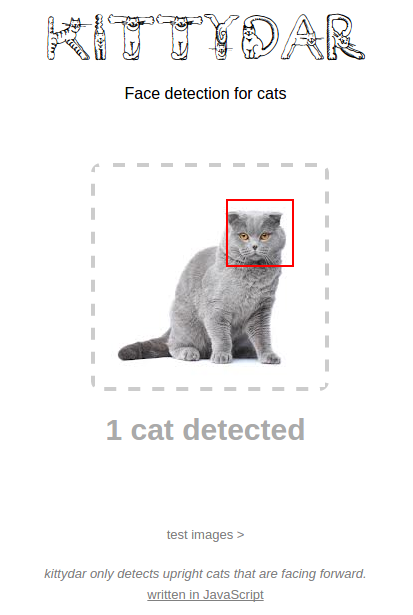
\includegraphics[scale=0.27]{imagen/Captura.png}
		\end{figure}
	\end{frame}
	\begin{frame}
		\frametitle{Reconocimiento facial de gatos.}
		%CONTENT
		Comparación entre métodos.
		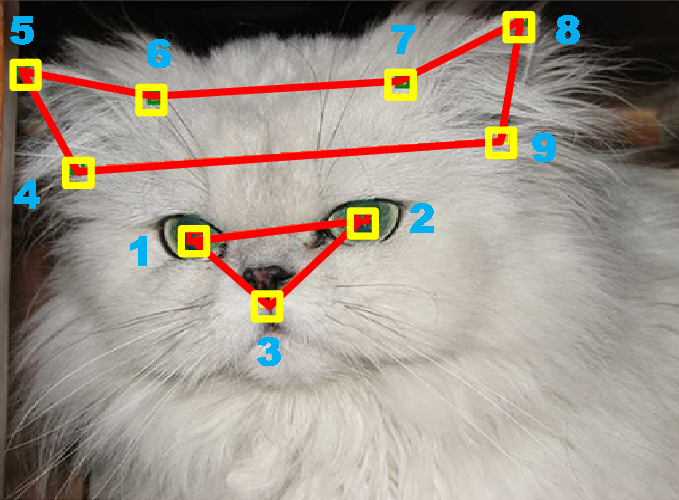
\includegraphics[scale=0.15]{imagen/annotation.png}
		\begin{itemize}
			\item{
				HOG.
			}
			\item{
				Haar.
			}
			\item{
				Detección de formas y textura conjunta.
			}
		\end{itemize}
		\begin{figure}[H]
			\centering
			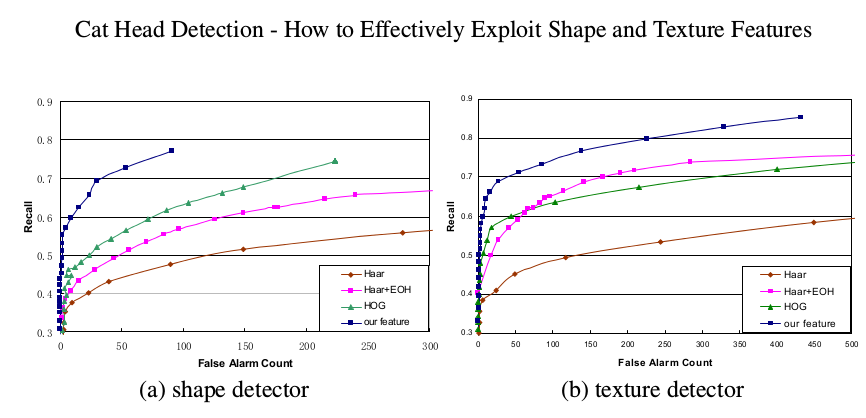
\includegraphics[scale=0.30]{imagen/cat-roc.png}
		\end{figure}
	\end{frame}
	\begin{frame}
		\frametitle{Resultados}
		%CONTENT
		\begin{figure}[H]
			\centering
			\subcaptionbox{}{
\includegraphics[scale=0.07]{imagen/nw1.jpg}}
			\subcaptionbox{}{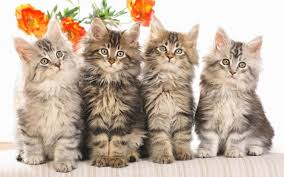
\includegraphics[scale=0.38]{imagen/nw2.jpg}}
			\subcaptionbox{}{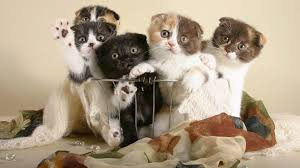
\includegraphics[scale=0.39]{imagen/nw3.jpg}}
			\caption{No reconoce gatitos.}
		\end{figure}
	\end{frame}
	\begin{frame}
		\frametitle{Resultados}
		%CONTENT
		\begin{figure}[H]
			\centering
			\subcaptionbox{}{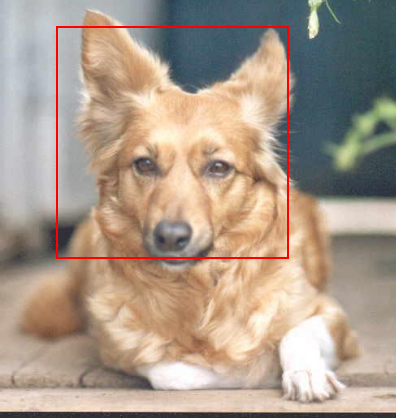
\includegraphics[scale=0.3]{imagen/w1.png}}
			\subcaptionbox{}{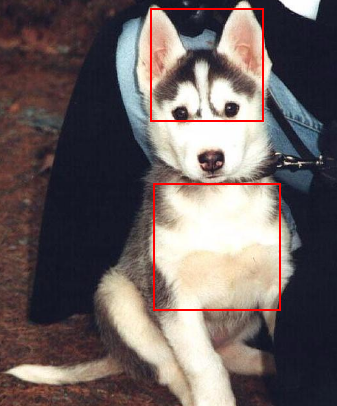
\includegraphics[scale=0.31]{imagen/w2.png}}
			\caption{Reconoce algunos perros.}
		\end{figure}
	\end{frame}
	\begin{frame}
		\frametitle{Resultados}
		%CONTENT
		\begin{figure}[H]
			\centering
			\subcaptionbox{}{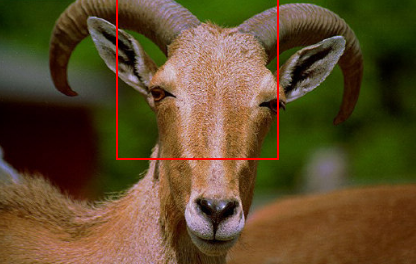
\includegraphics[scale=0.27]{imagen/f1.png}}
			\subcaptionbox{}{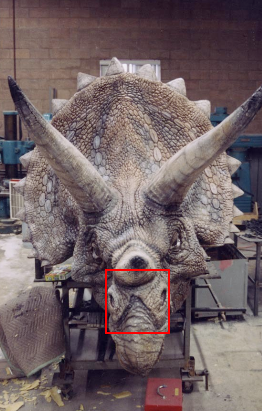
\includegraphics[scale=0.28]{imagen/f2.png}}
			\subcaptionbox{}{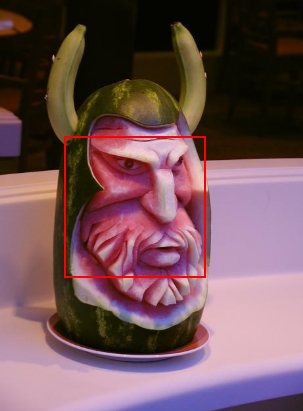
\includegraphics[scale=0.28]{imagen/f3.png}}
			\caption{Reconoce... cosas.}
		\end{figure}
	\end{frame}
	\begin{frame}
		\frametitle{Clasificación en Razas de Gatos y Perros.}
		%CONTENT
		\emph{Cats and Dogs}.\cite{parkhi12a}
		\begin{itemize}
			\item{
				HOG para reconocimiento de \emph{Forma}.
			}
			\item{
				\emph{Bag of Words} para reconocimiento de \emph{textura}.
			}
		\end{itemize}
		Combinaciones de Rostro, Cuerpo y Fondo.
		\begin{figure}[H]
			\centering
			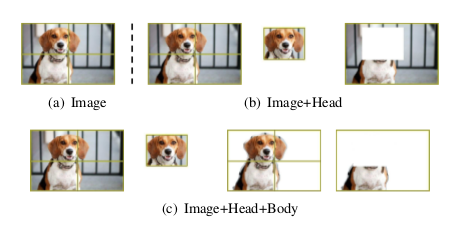
\includegraphics[scale=0.50]{imagen/faceheadimage.png}
		\end{figure}
	\end{frame}
	\begin{frame}
		\frametitle{Clasificación en Razas de Gatos y Perros.}
		%CONTENT
		\begin{figure}[H]
			\centering
			{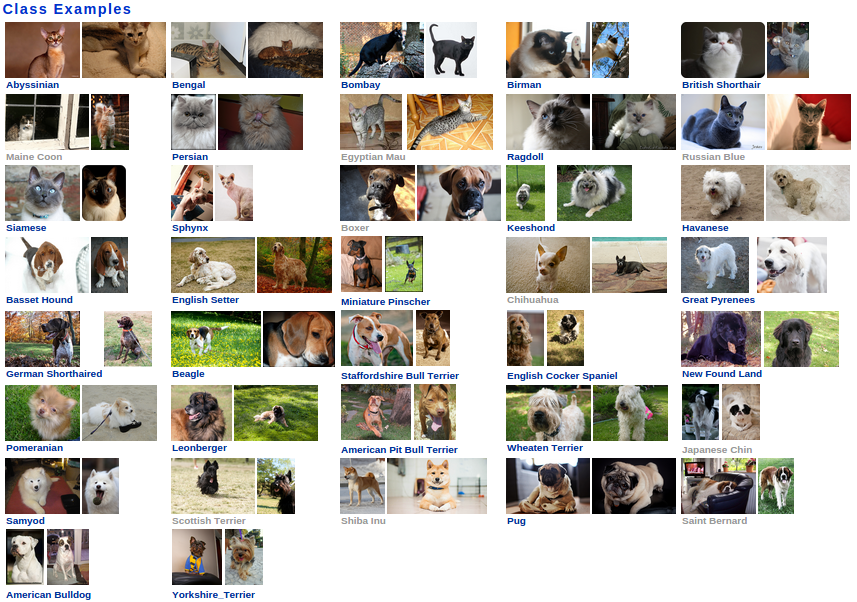
\includegraphics[scale=0.27]{imagen/datasetEx.png}}
			\caption{Dataset de razas de Perros y Gatos.}
		\end{figure}
	\end{frame}
	\begin{frame}
		\frametitle{Reconocimiento facial de Perros.}
		%CONTENT
		\emph{Biometric Recognition for Pet Animal}.\cite{kumar2014biometric}

		PCA \& Eigenfaces.
	\end{frame}
	\begin{frame}
		\frametitle{Reconocimiento facial de Perros.}
		%CONTENT
		\begin{figure}[H]
			\centering
			{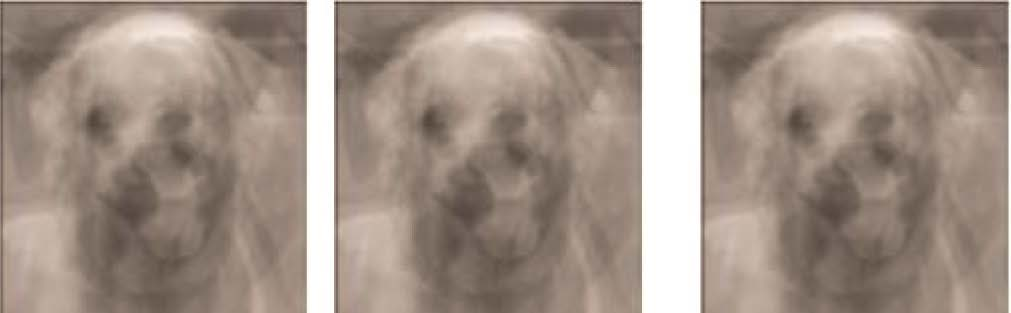
\includegraphics[scale=0.27]{imagen/dogaverage.png}}
			\caption{Eigenfaces para Perros.}
		\end{figure}
	\end{frame}

%COMENTARIO TERMINA ACA ==============================================================================
\end{comment}
\end{document}
